\documentclass[11pt,a4paper]{article}
\usepackage[margin=2.3cm]{geometry}
\usepackage{graphicx,booktabs,amsmath,hyperref,caption,subcaption}
\usepackage[T1]{fontenc}\usepackage{lmodern}
\hypersetup{colorlinks=true,linkcolor=black,urlcolor=blue}
\emergencystretch=3em\setlength{\parskip}{0.5em}\setlength{\parindent}{0pt}
\title{Budget-Aware Index Tuning with Wii and Esc on TPC-H (SF10):\\ Experimental Results}
\author{Databases course project -- interim report}
\date{22 November 2026}
\begin{document}
\maketitle

\begin{abstract}
We evaluate a budget-aware two-phase greedy index tuner and the Wii call-skipping mechanism (Wang et al., SIGMOD 2024) on TPC-H at scale factor 10, using PostgreSQL 18.7 with default planner settings. Wii finds indexes that improve the workload cost by 32.2\% using 429 what-if calls, against 33.4\% with 3092 calls for the same tuner without Wii (96\% of the quality with 14\% of the calls); at tight call budgets (500--1000) it is 3--7 points better than the budgeted baseline. The alpha parameter trades calls for quality smoothly, random skipping is far worse than Wii's bound-based skipping, and the cost model satisfies Wii's monotonicity and submodularity assumptions in more than 98\% of tested cases. Our implementation of Esc (Wang et al., PVLDB 2025), an early-stopping checker on top of the same tuner, saves 17--28\% of the calls at $K=20$ without measurable loss when used without Wii, but cannot stop when combined with Wii, because Wii's skipped calls leave its upper bound loose. Against the eight algorithms of the original study at about 10~GB, the tuner with Wii is within about 1 point of the best (CoPhy, DTA, Relaxation) using 429 calls where they use 1\,860--28\,102. The Wii results are single runs on one set of table statistics; the Esc results are repeated over two or three independent draws.
\end{abstract}

\section{Setup}
\textbf{Tuner.} The project's platform now contains a two-phase greedy algorithm (per-query greedy search, then greedy over the union of the selected indexes) running behind a cost oracle that counts and limits what-if calls. The oracle has four modes: \emph{none} (every cost question is answered by a what-if call until the budget is spent, after which the cheapest known cost of a subset of the configuration is used), \emph{Wii}, \emph{Wii + coverage} (a refinement of Wii's bounds) and \emph{random} (skips a call with fixed probability; used as a control). Wii skips a call when the lower bound $L$ on the query's cost under a configuration is within a factor $\alpha$ of the upper bound $U$ (the cheapest known cost of any subset), i.e.\ $L/U\ge\alpha$, and uses $U$ instead. The initial calls (no-index cost, and the cost with all candidates for Wii) count against the budget.

\textbf{Workload and environment.} TPC-H, SF10, 19 queries (2, 17 and 20 excluded, as in the platform's baseline experiments). PostgreSQL 18.7, HypoPG 1.4.5, all planner settings at their defaults (\texttt{max\_parallel\_workers\_per\_gather}=2, \texttt{work\_mem}=4\,MB, \texttt{shared\_buffers}=128\,MB, \texttt{random\_page\_cost}=4, \texttt{effective\_cache\_size}=4\,GB). Index width up to 2; the constraint is the number of indexes $K\in\{10,20\}$ with no storage limit. Table statistics were gathered once, with \texttt{ANALYZE}, and then frozen; the no-index workload cost is 42\,625\,951.

\textbf{Metric.} Improvement $=1-\text{cost}(\text{indexes})/\text{cost}(\emptyset)$, with the cost of the final configuration obtained by fresh what-if calls for every query (not from the tuner's own, possibly derived, numbers). ``Calls'' are what-if calls issued by the oracle; repeated questions and indexes irrelevant to a query are not counted.

\section{Results}
\subsection{Quality against call budget}
\begin{figure}[h]\centering
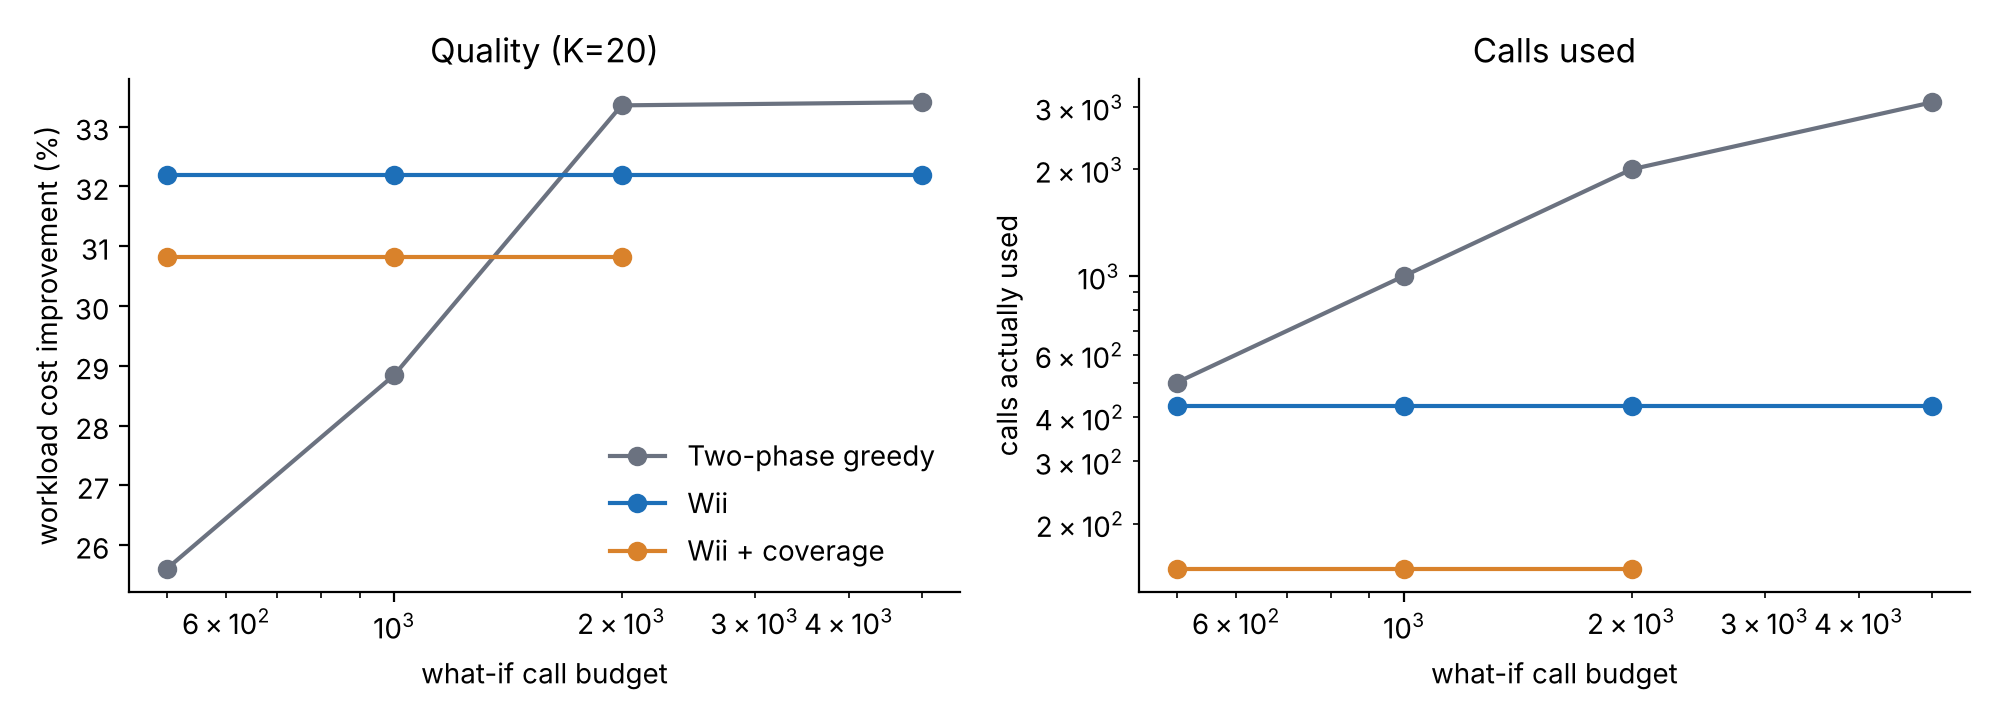
\includegraphics[width=\textwidth]{fig_budget.png}
\caption{Improvement (left) and what-if calls actually used (right) for $K=20$. Wii (alpha 0.9) always needs 429 calls and wii+coverage 149, so their curves are flat; the baseline is limited by the budget.}\label{fig:budget}
\end{figure}

\begin{table}[h]\centering\small
\begin{tabular}{lrrrr}\toprule
Budget $B$ & Baseline & Wii ($\alpha=0.9$) & Wii + coverage & Baseline calls\\\midrule
500 & 25.60\% & 32.19\% (429 calls) & 30.82\% (149) & 500\\
1000 & 28.84\% & 32.19\% & 30.82\% & 1000\\
2000 & 33.36\% & 32.19\% & 30.82\% & 2000\\
5000 (not binding) & 33.41\% & 32.19\% & -- & 3092\\\bottomrule
\end{tabular}
\caption{TPC-H SF10, $K=20$. For $K=10$ the Wii rows are identical and the baseline gives 25.60, 28.84, 32.40 and 33.01\% (2795 calls at $B=5000$).}\label{tab:main}
\end{table}

Wii is 6.6 points better than the baseline at $B=500$ and 3.4 points better at $B=1000$. At $B=2000$ the baseline, now with enough calls, overtakes it. Wii never uses more than 429 calls, so the larger budgets of this sweep do not constrain it: the four Wii entries in Table~\ref{tab:main} are one and the same run. A sweep of smaller budgets would be needed to see where Wii itself starts to degrade; the 38 initial calls set a lower limit.

\subsection{The role of alpha}
\begin{figure}[h]\centering
\begin{subfigure}{0.48\textwidth}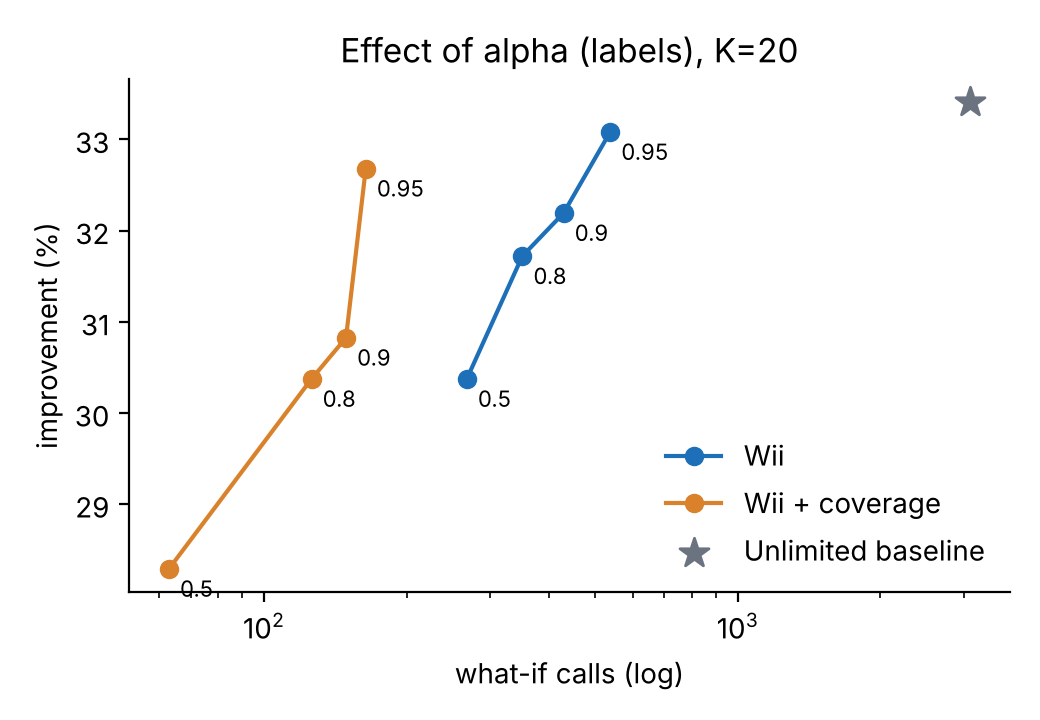
\includegraphics[width=\textwidth]{fig_alpha.png}\caption{Improvement against calls for different $\alpha$.}\end{subfigure}\hfill
\begin{subfigure}{0.48\textwidth}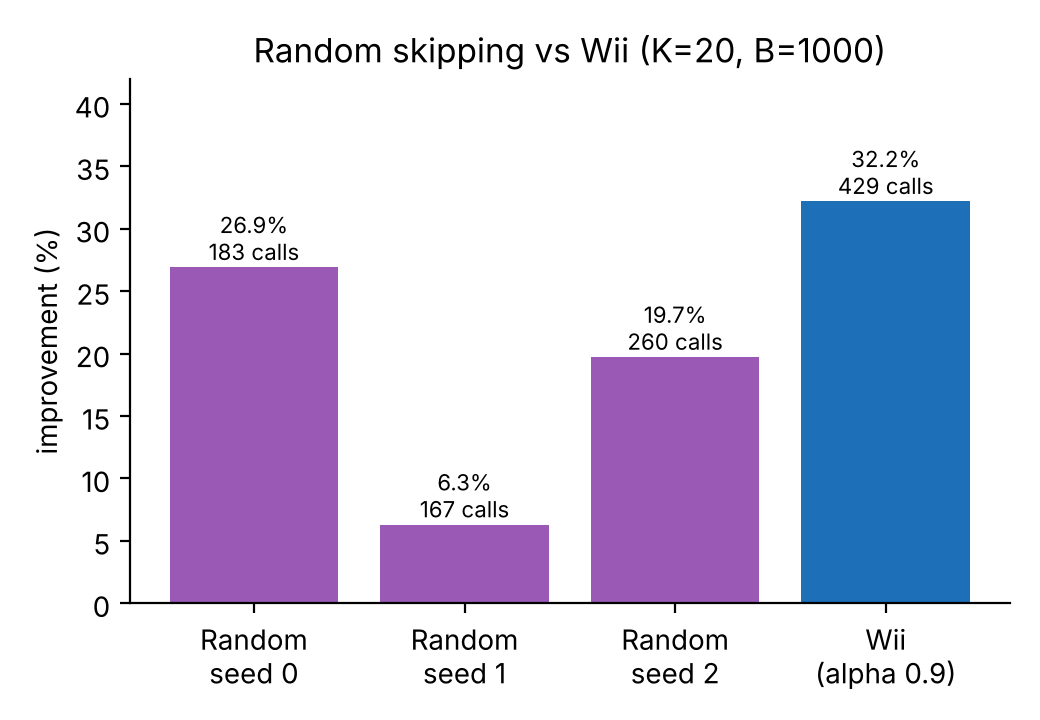
\includegraphics[width=\textwidth]{fig_random.png}\caption{Random skipping against Wii.}\end{subfigure}
\caption{Left: higher $\alpha$ skips fewer calls and gives better indexes. Right: random skipping at probability 0.9 with three seeds, against Wii.}\label{fig:alpha}
\end{figure}

\begin{table}[h]\centering\small
\begin{tabular}{lrrr}\toprule
$\alpha$ & Wii improvement (calls) & Wii + coverage (calls) & Wii quality vs.\ unlimited\\\midrule
0.5 & 30.37\% (268) & 28.29\% (63) & 90.9\%\\
0.8 & 31.72\% (351) & 30.37\% (126) & 94.9\%\\
0.9 & 32.19\% (429) & 30.82\% (149) & 96.3\%\\
0.95 & 33.08\% (538) & 32.68\% (164) & 99.0\%\\\bottomrule
\end{tabular}
\caption{Alpha sweep ($K=20$, $B=1000$); the unlimited baseline reaches 33.41\% with 3092 calls.}\label{tab:alpha}
\end{table}

With $\alpha=0.95$ Wii reaches 99\% of the unlimited baseline's improvement with 538 calls (17\% of 3092). The coverage refinement uses fewer calls at the same $\alpha$ but gives lower quality in every row on this workload.

\textbf{Random skipping.} Skipping 90\% of calls at random gives 26.9\%, 6.3\% and 19.7\% improvement for three seeds, using 167--260 calls, while Wii gets 32.2\% with 429. Which calls are skipped matters: Wii's bounds pick calls that carry little information, random skipping does not. The large spread between seeds (6--27\%) also means a single random seed would be misleading.

\subsection{Why skipping is safe: derived against real costs}
\begin{figure}[h]\centering
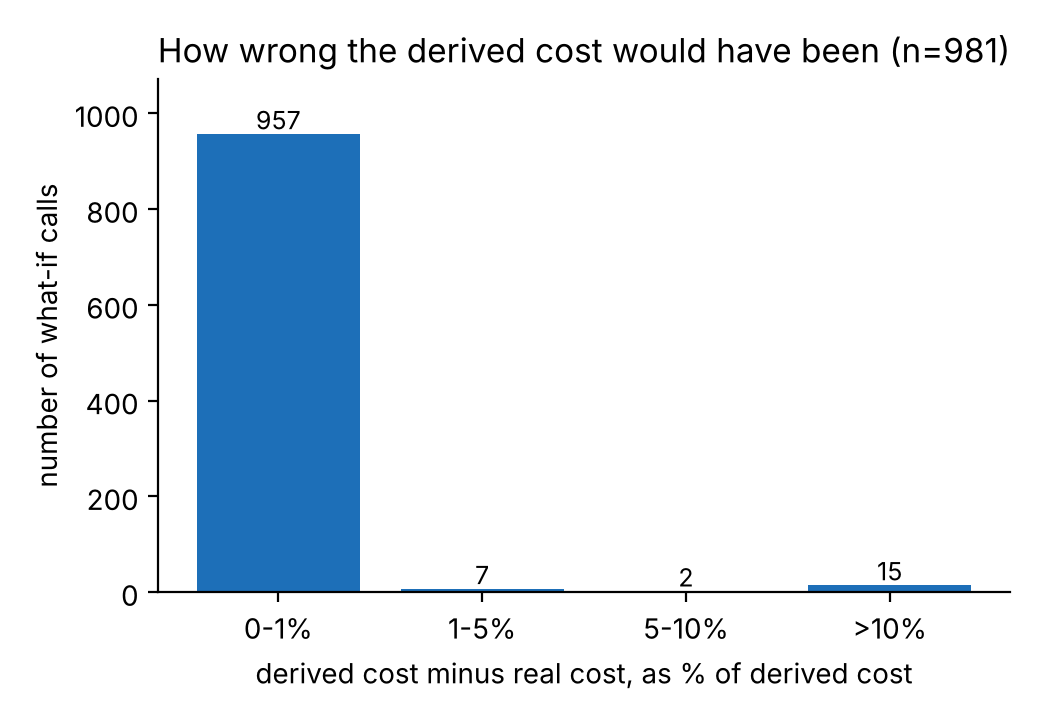
\includegraphics[width=0.55\textwidth]{fig_gaps.png}
\caption{For every real what-if call of a budgeted baseline run ($K=20$, $B=1000$), the error the derived cost would have had.}\label{fig:gaps}
\end{figure}
In 957 of 981 calls (97.6\%) the cost derived from already-known configurations is within 1\% of the real cost; only 15 calls (1.5\%) are off by more than 10\%. Most what-if calls of the baseline are therefore redundant, which is what Wii exploits.

\subsection{Assumptions of the cost model}
Wii's bounds rest on monotonicity (adding an index does not increase the cost) and submodularity (the benefit of an index does not grow when other indexes are present). Using the best single index of each query paired with each other candidate (643 pairs over 19 queries), PostgreSQL's cost model violates monotonicity in 3 pairs (0.5\%) and submodularity in 9 pairs (1.4\%). The worst monotonicity violation is query~8, where adding an index raised the estimated cost by 19\%. The violations are rare, which is consistent with Wii's small quality loss, but they mean the bounds are not guaranteed.

\section{Esc: early stopping}
\textbf{Implementation.} Esc-B (the variant without index interaction) is checked at the start of each greedy step of the second phase. It stops when $\eta_U-\eta_L\le\epsilon$: $\eta_L$ is the improvement of a simulated greedy completion that uses derived costs only; $\eta_U$ is Eq.~10 of the paper, the $K$ largest workload-level marginal-improvement bounds summed. On stopping, the simulated completion is returned. Esc-I, the generic rate-based filter and the MCTS variants are not implemented. A second, optional variant (``clamped'', our addition) additionally caps $\eta_U$ at the improvement obtained with all candidate indexes at once.

\begin{table}[h]\centering\small
\begin{tabular}{llrrrr}\toprule
$K$ & Variant & $\epsilon$ & Calls saved & Improvement lost & Guarantee\\\midrule
20 & plain Esc-B & 1--2\% & 16.9--19.8\% & 0.00 pts & yes\\
20 & plain Esc-B & 5--10\% & 24.3--27.8\% & 0.00 pts & yes\\
10 & plain Esc-B & 1--2\% & 8.9--9.9\% & 0.04 pts & yes\\
10 & plain Esc-B & 5--10\% & 17.1--18.8\% & 0.04--0.19 pts & yes\\
20 & clamped & 1--10\% & 33.3--37.5\% & 0.04--0.05 pts & no\\
10 & clamped & 1\% & 24.3--26.7\% & 0.13 pts & no\\
10 & clamped & 2--10\% & 27.0--29.8\% & 0.59--0.63 pts & no\\
20 & Wii + plain & any & 0.0\% & 0.00 pts & yes\\
20 & Wii + clamped & 1--10\% & 7.4--7.5\% & 0.00 pts & no\\
10 & Wii + clamped & 1\% & 1.9--2.1\% & 0.00--0.02 pts & no\\
10 & Wii + clamped & 2--10\% & 7.4--7.5\% & 0.09--0.11 pts & no\\\bottomrule
\end{tabular}
\caption{Esc on TPC-H SF10: calls saved and improvement lost relative to the same run that never stops (about 3\,000 calls without Wii and 430 with Wii at $K=20$). Ranges are over independent statistics draws (three for plain Esc-B, two for the clamped variants; no-index cost 42.59--42.69M).}\label{tab:esc}
\end{table}

\textbf{Without Wii.} Plain Esc-B saves 17--28\% of the calls at $K=20$ and 9--19\% at $K=10$ across three statistics draws, with at most 0.19 points of quality lost (none at $K=20$). The actual loss is far below the tolerated $\epsilon$ because the bound is loose (a gap of 2.6--3.0 points at the first check). Stopping points are coarse: a check happens only at Phase-2 steps, and for $\epsilon\gtrsim3\%$ the first check already passes. The check costs 0.03--0.08\,s.

\textbf{With Wii.} The plain checker never stops (430 calls in every run). Wii skips the calls that would give exact costs for the bound, so $\eta_U$ stays at 0.544 against $\eta_L=0.333$ after Phase~1 (from an earlier draw). Only about 36 of the calls come after Phase~1, so even a perfect checker could save at most about 8\%.

\textbf{Storage of the stopped configuration.} In all three draws the configuration returned by plain Esc-B at $K=20$ costs the same as the never-stopping run's (to 0.01 points) but swaps 2--3 of its 20 indexes for others, and takes 1.4--2.0\,GB (13--19\%) more space (10.3 against 12.3\,GB in the third draw). The simulated completion only sees derived costs, in which the swapped indexes are interchangeable, so it can pick larger ones. The paper's early stopping is about calls, so this is not a flaw in the bound, but it matters when storage is limited, and Esc would then need a storage-aware tie-break.

\textbf{The clamp is a heuristic.} With it, 7.4--7.5\% of calls are saved with Wii and 33--38\% without (two draws). But the clamp assumes that adding indexes never raises the estimated cost, and PostgreSQL does not guarantee that (see above): at $K=20$ without Wii the checker stopped with $\eta_L=0.3203$ above the clamped $\eta_U=0.3161$ (first draw), and in the second draw the violation counter registered one violation in each clamped $K=20$ run without Wii and none in any other run. The bound is then raised to $\eta_L$ and the event counted, so the clamped checker keeps no guarantee. In our runs the actual loss stayed below $\epsilon$ (at most 0.59 points, at $K=10$), but this is an observation, not a bound.

\section{Comparison with the eight algorithms of the original study}
The tuner's configurations are limited by the number of indexes $K$, not by storage, so each is compared with the baselines at the closest storage point of the original sweep (10\,GB budget; for AutoAdmin and Drop, which take an index count, $K=10$). The baseline numbers are means over three repetitions of the platform's runs on PostgreSQL 18.7 (same defaults, separate statistics draw), with a spread over repetitions of up to 1--3 points (CoPhy 2.5, DTA 3.2), so differences below about 2 points should not be read as a ranking.

\begin{table}[h]\centering\small
\begin{tabular}{llrrr}
\toprule
Algorithm & Setting & Rel.\ cost \% & What-if calls & Runtime s\\
\midrule
Extend & 10 GB & 70.5 & 2552 & 3.9\\
Relaxation & 10 GB & 67.6 & 1860 & 3.6\\
DTA & 10 GB & 67.6 & 28102 & 52.5\\
CoPhy & 10 GB & 66.3 & 23066 & 13.8\\
DB2Advis & 10 GB & 70.0 & 38 & 0.1\\
AutoAdmin & K=10 & 67.7 & 2671 & 3.9\\
Drop & K=10 & 72.2 & 1066 & 2.5\\
Two-phase greedy & K=20, 10.3 GB & 66.6 & 3092 & 4.5\\
Wii ($\alpha{=}0.9$) & K=20, 9.9 GB & 67.8 & 429 & 0.7\\
Wii + coverage & K=20, 10.6 GB & 69.2 & 149 & 0.3\\
Two-phase + Esc-B (5\%) & K=20, 12.3 GB & 67.6 & 2179 & 3.3\\
\bottomrule
\end{tabular}

\caption{Relative workload cost (lower is better), what-if calls and runtime at about 10\,GB. Dexter (no what-if calls; 10\% threshold) reaches 70.7\%. The Esc row comes from a different statistics draw, whose own never-stopping run gave 67.6\%, 3\,016 calls and 10.3\,GB.}\label{tab:compare}
\end{table}

\begin{figure}[h]\centering
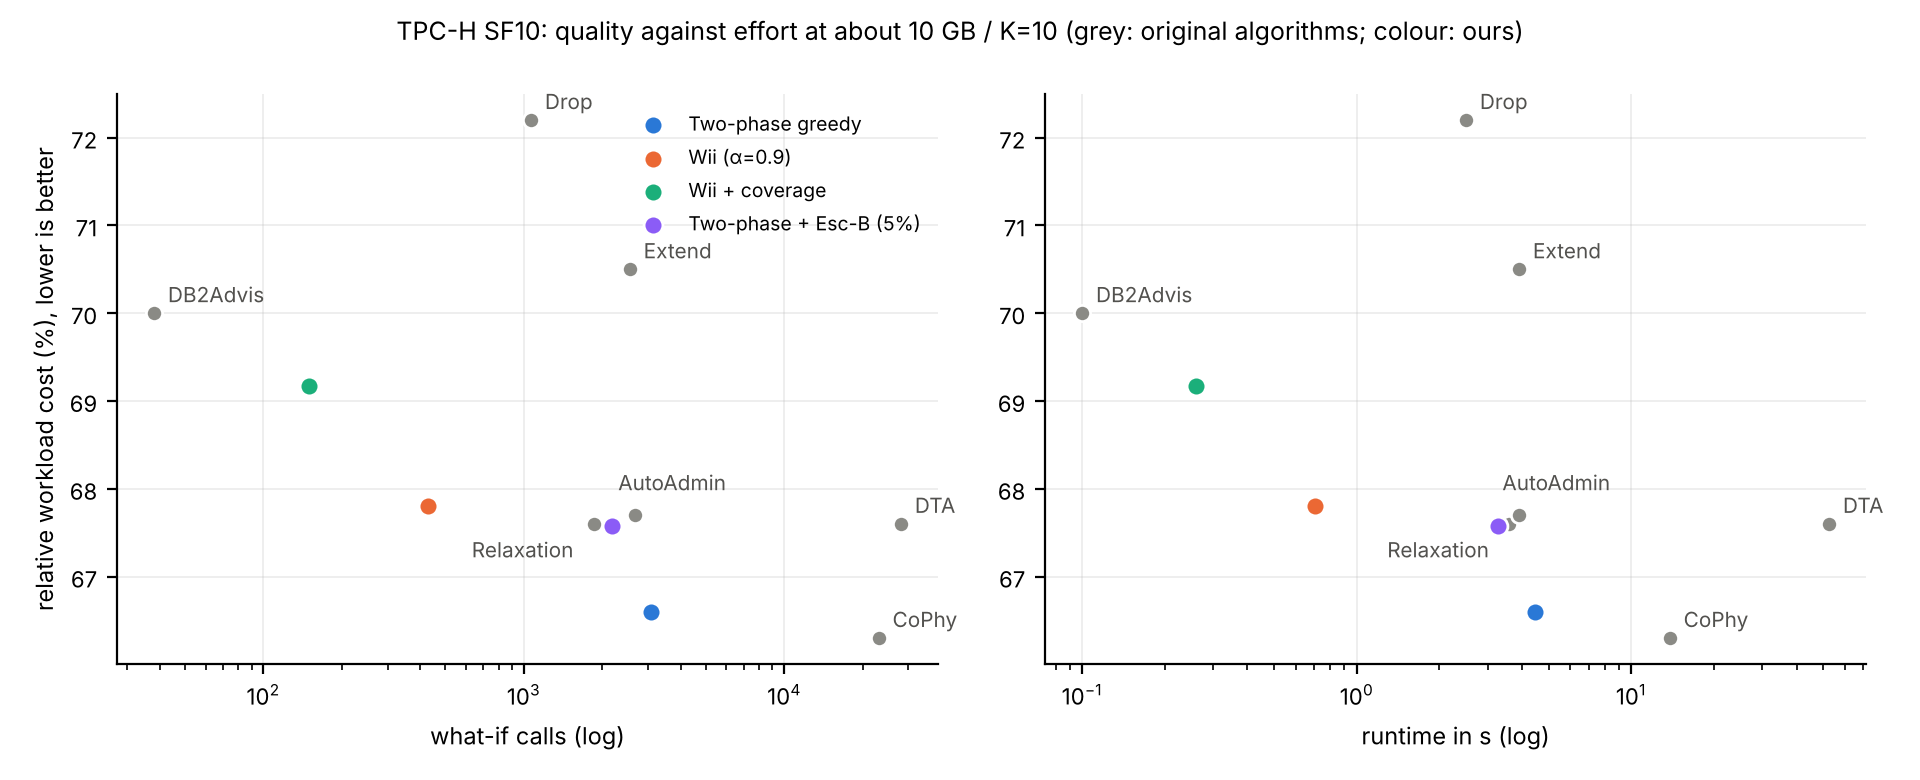
\includegraphics[width=\textwidth]{fig_compare.png}
\caption{Relative workload cost against what-if calls (left) and runtime (right).}\label{fig:compare}
\end{figure}

Wii reaches 67.8\%, within 1.5 points of CoPhy (66.3\%) and level with Relaxation, DTA and AutoAdmin (67.6--67.7\%), with 429 calls against 1\,860 (Relaxation), 2\,671 (AutoAdmin), 28\,102 (DTA) and 23\,066 (CoPhy). It beats Extend (70.5\%), Drop (72.2\%), DB2Advis (70.0\%) and Dexter (70.7\%). Only DB2Advis (38 calls) uses fewer calls, and it is 2.2 points worse. The two-phase tuner without Wii (66.6\%, 3\,092 calls) is the best of everything except CoPhy, at 13\% of CoPhy's calls. Esc-B (5\%) cuts the tuner's calls to 2\,179 (28\% fewer in that draw) at the same cost, but see the storage remark above. Caveats: our tuner uses index width 2 and a count limit rather than a storage limit, the baselines were run with the original study's configuration, and calls are counted by different code paths (the platform's cost-request counter for the baselines, the oracle's calls for ours).

\section{Discussion and limitations}
\begin{itemize}
\item \textbf{Single statistics draw (Wii results and comparison).} Table statistics come from a random sample, and different \texttt{ANALYZE} runs move the no-index cost by about 0.1\% and the improvement of a run by up to 1--2 points (seen in earlier unfrozen runs: 32.95\% against 31.79\% for the same unlimited baseline). We froze the statistics, which makes runs repeatable but hides this spread; the conclusions above are about differences of several points, but differences below about 1--2 points (for example between alpha 0.9 and 0.95 coverage variants) should not be over-read.
\item \textbf{Planner settings.} A teammate's run with \texttt{max\_parallel\_workers\_per\_gather}=8 gave a lower cost scale (no-index cost $\approx$34.95M) and, as reported to us, the same qualitative patterns; we did not verify those runs and report only the default-settings results here.
\item \textbf{Estimated, not executed, costs.} As in the original platform, costs are optimizer estimates for hypothetical indexes; queries were not executed.
\item \textbf{Comparison with the paper.} The paper evaluates on other DBMS and workloads, with a different cost scale, so absolute improvements are not comparable; our results agree qualitatively with its motivation (many what-if calls are redundant; skipping them by bounds keeps most of the quality; budget reallocation helps most when the budget is tight). We did not reproduce its numbers.
\item \textbf{One workload.} Only TPC-H at SF10 so far; TPC-DS is configured but not run.
\end{itemize}

\section{Status and next steps}
\textbf{Done:} Wii on TPC-H SF10 with the alpha, random-skipping, gap and assumption experiments; Esc-B with its clamped variant and the analysis of why it cannot stop with Wii; the comparison with the eight original algorithms at about 10\,GB; plain Esc-B repeated over three independent \texttt{ANALYZE} draws (clamped: two).

\textbf{Still open:} (0) A storage-aware tie-break for the simulated completion (see above). (1) The Wii experiments themselves, including the comparison, rest on one statistics draw; repeat them over three draws and report the spread. (2) Add a sweep of small budgets (about 50--400) so that the budget limits Wii. (3) Run Esc under a limited call budget, where stopping early frees budget for something else. (4) Run the comparison with matched storage limits for our tuner. (5) Implement Esc-I and run TPC-DS.

\section*{Reproducibility}
Repository \texttt{RameezWahid/magic-mirror-revisited}, \texttt{main} (two-phase greedy and Wii: \texttt{selection/budget\_aware.py}, \texttt{selection/algorithms/two\_phase\_greedy\_algorithm.py}, \texttt{scripts/wii\_experiments.py}). Esc: branch \texttt{esc} (\texttt{selection/esc.py}, \texttt{scripts/esc\_summary.py}, \texttt{tests/test\_esc.py}), delivered as three patches. Command: \texttt{wii\_experiments.py configs/tpch\_sf10\_load.json <out> assumptions gaps wii alpha random unlimited}, and \texttt{... <out> esc esc\_clamp} for Esc; the baseline numbers come from the platform's \texttt{RESULTS.txt}; run data in \texttt{runs\_rep1.jsonl} and \texttt{assumptions.json}. Three repetitions gave identical results except one coverage run (164 or 165 calls, cost difference 10 out of $2.9\cdot10^7$), likely from floating-point summation order.

\section*{References}
\begin{enumerate}\small
\item X.\ Wang, W.\ Wu, C.\ Wang, V.\ Narasayya, S.\ Chaudhuri. Wii: Dynamic Budget Reallocation In Index Tuning. SIGMOD 2024 (PACMMOD 2(3)).
\item X.\ Wang, W.\ Wu, V.\ Narasayya, S.\ Chaudhuri. Esc: An Early-Stopping Checker for Budget-aware Index Tuning. PVLDB 18(5), 2025.
\end{enumerate}
\end{document}
